\section{Hardness of Water}

\begin{multicols}{2}


\section*{Concept of Hardness of Water}


\subsection{Is the Water Pure?}
\label{sub:water-pure}

\begin{center}
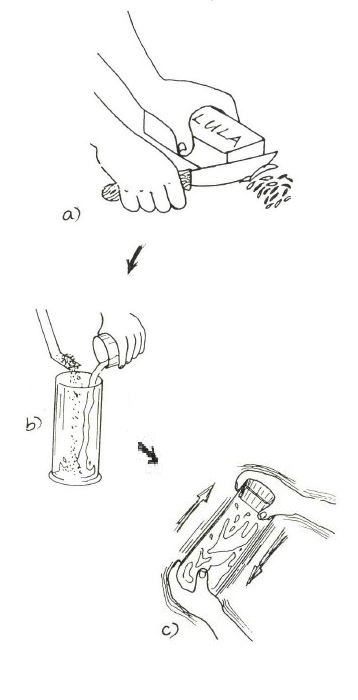
\includegraphics[width=0.4\textwidth]{./img/source/hard-water.jpg}
\end{center}

\begin{description*}
%\item[Subtopic:]{}
\item[Materials:]{2 bottles, tap water, rain water, soap}
%\item[Setup:]{}
\item[Procedure:]{Fill one bottle with tap water and another with distilled water (rain water). Add equal amounts of soap into each and shake well. }
%\item[Hazards:]{}
%\item[Questions:]{}
\item[Observations:]{Soft water foams easily, but hard
water will form a scum (white precipitate) and
little foam. Distilled water, because it is soft,
will foam easily.}
\item[Theory:]{Hard water is caused by dissolved solids.
However, a part of the hardness can be removed
by boiling. Hence, if hard tap-water is boiled, it
can become softer.}
%\item[Applications:]{}
%\item[Notes:]{}
\end{description*}


%==================================================================================================%

\section*{Types of Hardness of Water}


\subsection{Temporary and Permanent Hardness}

%\begin{center}
%\includegraphics[width=0.4\textwidth]{./img/.png}
%\end{center}

\begin{description*}
%\item[Subtopic:]{}
\item[Materials:]{Bottles, syringes, soap, Epsom salt (magnesium sulphate), bicarbonate of soda (sodium hydrogen carbonate), \nameref{sec:heatsources}, rain water, filter paper, funnel, washing soda (sodium carbonate)}
\item[Setup:]{In one bottle add a spoonful of Epson salt with 2 spoons of bicarbonate of soda and water. Stir until the salts dissolve. In a second bottle add a spoonful of Epsom salt with water and stir until dissolved. In a third bottle add rain water. Label the bottles ``temporary hard water,'' ``permanent hard water'' and `soft water,'' respectively. Prepare a separate sodium carbonate solution by dissolving 2 spoons of washing soda into 500 mL of water.}
\item[Procedure:]{In 3 separate syringes put approximately 5 mL samples of each solution, add soap and shake vigorously. Repeat but instead add a few drops of sodium carbonate solution. Boil a small amount of both temporary and permanent hard water. To the boiled permanent hard water, add a few drops of sodium carbonate solution. Filter the precipitate from the bolied temporary hard water and add a few drops of sodium carbonate.}
%\item[Hazards:]{}
%\item[Questions:]{}
%\item[Observations:]{}
\item[Theory:]{Magnesium sulphate mixes with sodium hydrogen carbonate solution to produce  an aqueous solution of magnesium hydrogen carbonate (temporary hard water). Magnesum sulphate solution is permanent hard water. When the temporary hard water is boiled, a white precipitate of magnesium carbonate should be observed. Boiling the permanent hard water will not cause precipitation.
The precipitation occurs because the hydrogen carbonate decomposes on boiling to form a carbonate which then precipitates with magnesium ions.\\
On boiling: 
\begin{center}
\ce{CO3^{2-}_{(aq)} + Mg2+_{(aq)} -> MgCO3_{(s)}}
\end{center}
After boiling and filtering, the sodium carbonate can indicate the presence or lack of magnesium ions. In the soft water and the boiled, filtered temporary hard water, no precipitate will be observed because there is no magnesium ion is present. In the permanent hard water, a precipitate will be observed with sodium carbonate}
%\item[Applications:]{}
%\item[Notes:]{}
\end{description*}

%==================================================================================================%

\section*{Treating Hard Water}


\subsection{Removing Hardness}

%\begin{center}
%\includegraphics[width=0.4\textwidth]{./img/.png}
%\end{center}

\begin{description*}
%\item[Subtopic:]{}
\item[Materials:]{Rock soaked in hard water, vinegar, water, bucket}
%\item[Setup:]{}
\item[Procedure:]{Place a rock or other object with hard water remains on it in a bucket. Add equal parts vinegar and water to cover the object and let it sit overnight.}
%\item[Hazards:]{}
%\item[Questions:]{}
\item[Observations:]{The remains of the hard water will dissolve.}
\item[Theory:]{Hard water contains dissolved magnesium or calcium ions.
Soft water does not. Calcium and magnesium carbonates dissolve easily in vinegar, and it is difficult to dissolve them back into water.}
%\item[Applications:]{}
%\item[Notes:]{}
\end{description*}

\subsection{Effect of Soda on Hard Water}

\begin{center}
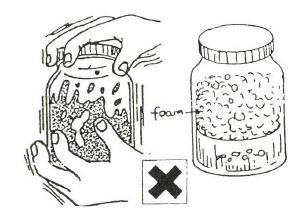
\includegraphics[width=0.4\textwidth]{./img/source/soda-hard-water.jpg}
\end{center}

\begin{description*}
%\item[Subtopic:]{}
\item[Materials:]{Water, soap, bottle, washing soda (sodium carbonate)}
%\item[Setup:]{}
\item[Procedure:]{Add some ash extract or washing soda to tap water and shake well. Filter and add soap and shake as described in \nameref{sub:water-pure} (p.~\pageref{sub:water-pure}).}
%\item[Hazards:]{}
%\item[Questions:]{}
\item[Observations:]{A lot of foam is formed this time.}
\item[Theory:]{The water has been softened by this process.
The soda (sodium carbonate) precipitates
the Ca$^{2+}$ and the Mg$^{2+}$ ions (which cause the
hardness) as the respective carbonates which
are filtered off.}
%\item[Applications:]{}
%\item[Notes:]{}
\end{description*}

%==================================================================================================%



\end{multicols}

\pagebreak